\chapter{Representative State Transfer (REST)}
\label{chap:rest}

\lstset{frame=none,
  language=JAVA,
  aboveskip=3mm,
  belowskip=3mm,
  showstringspaces=false,
  columns=flexible,
  basicstyle={\small\ttfamily},
  numbers=none,
  breaklines=false,
  breakatwhitespace=false,
  tabsize=3
}

\section{REST architecture}
\label{sec:rest-architecture}

REST is "a set of constraints on the overall architectural approach" \cite{agile-architecture}. Roy Thomas Fielding described REST in his doctoral dissertation as an architectural style. The constraints are applied to obtain desired properties of developed architecture. REST is applicable to \gls{hypermedia} applications where multimedia nodes are connected via hyperlinks.

REST architecture is client-server. The server holds implemented logic of services and encapsulates it under the interfaces. The interfaces are entry points for client. Through them data can be obtained and modified. 

\begin{figure}[htp] \centering{
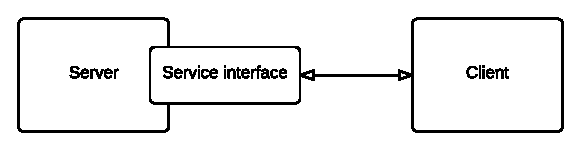
\includegraphics[width=8cm]{img/communication-through-interface.pdf}}
\caption{Client enter the server through the interfaces}
\label{fig:communication-through-interface}
\end{figure} 


The REST is \gls{resource-based-model}. It operates resources named by nouns and actions are provided by HTTP requests. 
REST architecture is a composition of \emph{elements}, \emph{connectors} and \emph{components}. None of them defines specific technology, they are abstractions. The elements abstract a behaviour of components. The components have their roles, the way of interaction among them and interpretation. The REST coposition will be described in Section \ref{sec:rest-composition}

REST has its best practices and constraints. Only services which are built according to this definition can be called \emph{RESTful}. Six constraints characterizing the REST will be described further in Section \ref{sec:constraints}.

\section{Composition of REST}
\label{sec:rest-composition}
As was mentioned above, REST architectional style consist of data elements, connectors and components, shown in Figure \ref{fig:composition-rest}. REST is resource-based, so the main data element is a resource. It is accompanied by resource metadata. Next elemetns are represenatation and its metadata. The last set od data elements are control data. Other than elements REST consists of connectors and components.

\begin{figure}[htp] \centering{
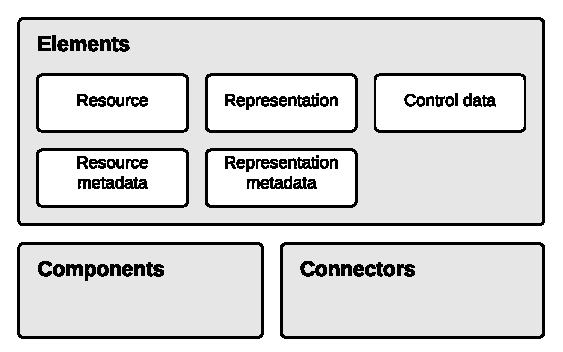
\includegraphics[width=8cm]{img/composition-rest.pdf}}
\caption{Composition of REST}
\label{fig:composition-rest}
\end{figure} 

\subsection{Data elements}
\subsubsection{Resource}
  Resource is an abstraction of information. Any information which can be named by noun can be a resource. "A resource is a conceptual mapping to a set of entities.." \cite{fielding} or set of values. The values can be resource identifiers and representations.
  Resource can be static (for example \emph{an image}) or dynamic (\emph{the time} which dynamically changes).
  
  Examples:
  \begin{center} 
  \begin{lstlisting}
      customer, 
      account, 
      order, 
      ..
  \end{lstlisting} 
  \end{center}

\subsubsection{Resource identifier}
  Serves to identify resources. The resource identifier is assigning a name thanks to which it is possible to reference appropriate resource. The identifier is \gls{url}. It marks a path to reach the resource. A request from client is routed to the specific service and method.
It should be possible to perform the \gls{CRUD} operations with the resources, every operation can be mapped on HTTP method. Having the method and the path the specific operation is performed.

Examples: \\
\begin{center}
\begin{tabular}{l l l}
Method & URL Path & Operation performed \\ \hline
GET & /customers & Retrieves all customers \\
GET & /customers/5 & Retrieves customer with id 5 \\
POST & /customers & Creates new customer \\
PUT & /customers/13 & Updates customer with id 13 \\
DELETE & /customer/2 & Deletes customer with id 2 \\
\end{tabular}
\end{center}

\subsubsection{Representation}
  Representation is used by REST components to perform changes to the resource. The representation stands for a part of (less commonly the whole) resource state. Format of representation's data is called media type and affects the performance of the \gls{hypermedia}. Media types can be proprietary or standardized, from standardized types. There are for comparison \gls{xml} and \gls{json}. JSON format is less verbose and smaller than XML and in consequence in sake of data transmission it would perform faster than a XML representation format.
  
Example of representation:
\begin{center}
  \begin{tabular}[b]{l l}
    In XML format & \begin{lstlisting}
    <?xml version="1.0" encoding="utf-8">
    <customer> 
      <name>Peter<\name> 
      <surname>Smith<\surname> 
      <dateofbirth>20-4-1975<\dateofbirth> 
    <\customer>
    \end{lstlisting} \\
    
\\
    
    In JSON format & \begin{lstlisting}
    {
        "name": "Peter", 
        "surrname": "Smith", 
        "dateofbirth": "20-4-1975"
    }
    \end{lstlisting}
  \end{tabular}
\end{center}

\subsubsection{Representation metadata}
  Representation metadata describes the data of which the representation consists. For example Content-Type defines the \gls{mime-types} of representation sent between client and server. Last-Modified defines the date of last modification of requested object.

  \begin{center}
  \begin{lstlisting}
    {Content-Type: application/json}
    {Content-Type: application/xml}
    {Last-Modified: Thu, 19 May 2015 21:58:55 GMT}
    
  \end{lstlisting}
  \end{center}
  
\subsubsection{Resource metadata}
  Resource metadata describes resources. The examples are Vary which comunicate with proxies whether use a cashed response or request a new ono. Other example is Allow. It defines the allowed methods for a specified resource.
  
  \begin{center}
  \begin{lstlisting}
    {Vary: *}
    {Allow: GET}
  \end{lstlisting}
  \end{center}
  
\subsubsection{Control data}
  "Control data defines the purpose of a message between components, such as the action being requested or the meaning of a response." \cite{fielding}. It can control the caching and parametrize requests. An example can be If-Modified-Since which allows to return a specified response message (304 Not Modified)
  
  \begin{center}
  \begin{lstlisting}
    {If-Modified-Since: Thu, 16 Jun 2014 20:31:00 GMT}
  \end{lstlisting}
  \end{center}
  
  

To summarize the REST elements, every resource has its representation which describes how are resources manipulated in RESTful \gls{api} architecture. The representation is a part or whole resource state. It is transferred between the client and server and has generaly JSON or XML format, but could be in many other formats as well. Representations and resources have their metadata which describe them. Control data affects the messages between client and server.

Client sends a message to server when he wants to operate with a resource. This message is a request. It contains a resource identifier which locates the resource. The request has headers filled by metadata describing the resource and representation. And the body of request involves a representation. An example of a request to create a new customer.

Request:
\begin{center}
  \begin{lstlisting}
     POST /cutomer HTTP/1.1
     Content-Type: application/json
     If-Modified-Since: Thu, 16 Jun 2014 20:31:00 GMT

     {
        "name": "Peter", 
        "surrname": "Smith", 
        "dateofbirth": "20-4-1975"
     }
  \end{lstlisting}
  \end{center}
  
Response:
  \begin{center}
  \begin{lstlisting}
     HTTP/1.1 200 OK 
     Content-Type: application/json
     Allow: POST
     
     {
        "id": 23, 
     }
  \end{lstlisting}
  \end{center}
  
     
The client want to save a representation of customer to the resources. Resources are accessed by URL. Headers are consisting of representation content type which is JSON and control data of modification since specified date. The response message contains headers with content type of a representation and method which is allowed by resource metadata. The response returned an id of created customer. 





\subsection{Connectors}
The connectors encapsulate transfer of representations and access of resources. Connectors are: client, server, cache, resolver, tunnel. %TODO explanation, maybe image

\subsection{Components}
REST components are an abstraction of application unit. The components are origin server, gateway, proxy, user agent. %TODO explanation, maybe image

\section{REST constraints}
\label{sec:constraints}

The REST architectural style has to be developed with respect to its constraints. They are applied to an architecture to create RESTful services. This rules leads to desirable properties of the system, such as performance, scalability, simplicity, modifiability, visibility, portability and reliability. Constraints described below were defined by Roy Thomas Fielding and there are six of them in total.
%%(citacia http://www.restapitutorial.com/lessons/whatisrest.html#)
 
%TODO write about HATEOAS

\subsection{Uniform Interface}
  
Interface stands between client and server. Through the interface client access the server. The REST interface is uniform, client and server always use a fixed set of methods to provide operation over the resources. REST uses \emph{\gls{http} specification}, mostly GET, POST, PUT and DELETE verbs. Despite REST can work with other protocols and define different verbs it uses HTTP operations for practical purpposes. This concept than separates client and server allowing them to develop each part independently and to reduce the coupling between them. %The interface is uniform, so that is easy to understand for both, the server and the client.

Interface is resource-based. Resources are on the server side and the client sents a request process either create, get, update or delete operation over the resource. The request contains a resource identifier in \gls{uri}. It identifies a path to concrete resource. Depending on the type of the request, represention is sent from the client in request and/or from the server in response. The representation is conceptually separated from the resource. It represents appropriate database record.

Resources are manipulated exclusively through the representations. The representation with any metadata attached keeps enough information to modify the resource on the server.

%Sent message represents a clients request or a servers response and it is self-descriptive. It means there is enough information to know how to process the message and the response explicitly defines the cashability.

The representation is sent in a request using HTTP verbs (GET, POST, PUT, DELETE,..) and the URI. Server sends to the client a HTTP response. For illustration a simplified HTTP request and response format is shown in Figure \ref{fig:http}.

\begin{figure}[htp] \centering{
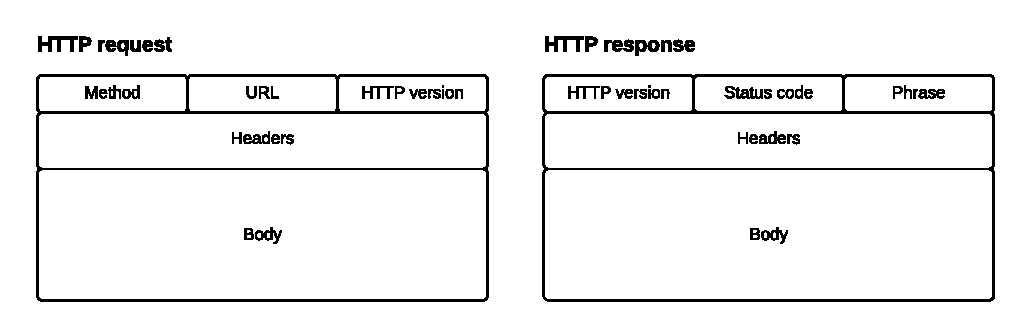
\includegraphics[width=12cm]{img/HTTP.pdf}}
\caption{HTTP request and response}
\label{fig:http}
\end{figure} 

Firts line in the request is called request line. It contains a name of method to be executed over the resource, the URL and HTTP version to be used. Then there are headers and the body for a representation. The response has the fist line starting with HTTP version, than there is a status code with appropriate phrase. Status and phrase reporting whether the request was successful or not.

\subsection{Stateless}
  
Each message is self-descriptive. Request has enough context to be understood and the messages have no state. Any state of a \gls{session} is held just on the client side (for example a logged-in user's session).
The statelessness allows greater scalability, because server doesn't have to communicate with the session, which can be created to carry the state using another architectural style of services. Reliability is improved because of easier recovery of partial failures. Disadvantage is that the sent requests contain repetitive data and the server has lower control over the application's behaviour.

\subsection{Client-server}

RESTful architecture is client-server oriented. There are two separate concerns. It is properly defined what is consumer's side and what are services on server side. Client can’t have direct access to the database, assets or resources. Client-server architecture improves portability of both client and server codes because they are standing alone. The architecture provide simplicity and scalability of server-side code because it doestn't have to include user interface. Client and server are linked together thanks to unified interface and the two can be developed independently.

\subsection{Cacheable}

Server responses (representations) are cacheable. They can be stored to eliminate the interactions with server . Responses can be defined as cashable implicitly, explicitly or negotiated. The cache can be established on server-side, client-side or both as can be seen on Figure \ref{fig:cacheability}. The reason for caching is to reduce interactions over the network. Cached responses are loaded from the cache instead of sending a request to the server. 
Cacheing partially decreses the client-server interaction but improves the scalability and performance. 


\begin{figure}[htp] \centering{
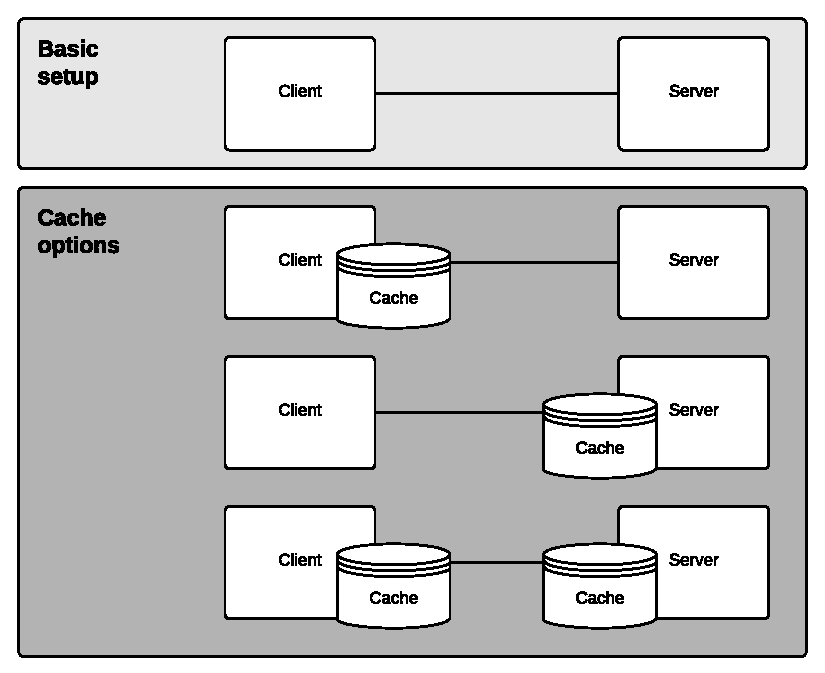
\includegraphics[width=10cm]{img/cacheablity.pdf}}
\caption{Cacheability options}
\label{fig:cacheability}
\end{figure} 

\subsection{Layered system}

This constraint is linked to cashability and client-server principle. System is composed of layers which rapresent independent parts of the system. Example of vertically layered system is shown on Figure \ref{fig:layered-system}. Client is not able to see whether he is communicating directly with the server, or with an intermedia between them. Intermedia improves scalability, provide shared caches and moreover can enforce security policies.

\begin{figure}[htp] \centering{
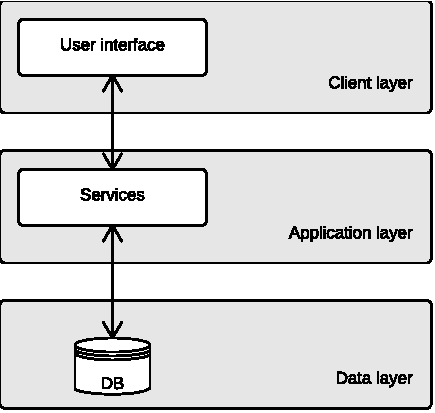
\includegraphics[width=7cm]{img/layered-system.pdf}}
\caption{Layered system example}
\label{fig:layered-system}
\end{figure} 

\subsection{Code on demand}

The logic can be transferred to the client-side. This way the server can temporarily extend or customize the functionality of the client. This can be performed for example by the components like service-side scripts.
This constraint is unique, it is the only one which can be violated and the services can be still RESTful.

\section{Application of REST}

Having the SOA and knowing the constraints of the REST services can be designed. When a company wants to develop a system with RESTful services it has to apply at least the first five constraints. But it can happen that not all the constraints are profitable for an application. In this case the architecture can skip some of them. In this case services cannot be further marked as RESTful. This notation doesn't affect services themselves, the result can be still the best design for current application. The RESTful services and their constraints are one of the possible solutions of architectural style. They are not the universal solution for system architecture.

\subsection{RESTful service example}
There is a company with SOA and its services are designed according to REST constraints. One of the services represents business abstraction of \emph{customers} of the company. Customers can be viewed, created, modified or deleted. The HTTP verbs (GET, POST, PUT, DELETE) are used to perform the operations. 

In designing the service there is considered the notation of \gls{webapi} \gls{framework}. 

Resource identifier is an \gls{url} address. ASP.NET Web API is composed of \emph{controller} and an \emph{action}. The controller is a class handling the HTTP request and the action is a method of the controller. In this example the action is \emph{GET}, the controller is \emph{customers} and to identify a specific customer there is a parameter \emph{name}. The template for GET operation look like:

\begin{lstlisting}
    GET     customers/{name} 
\end{lstlisting}


The URI identifies specific resource - \emph{customers}. Thanks to paramenter \emph{\{name\}} the request is performed on specific representation of resource. The parameter \emph{\{name\}} is a tepmlate. When the client wants to get the customer whose name is \emph{Peter} then the template is replaced

\begin{lstlisting}
    GET     customers/Peter 
\end{lstlisting}

The representation of customers with the neame Peter is retrieved. It has its media type which is stated in metadata. Content-Type header is dealing with the format of data sent in the requests and response.

\begin{lstlisting}
    Content-Type: application/json
    
    { 
    "name": "Peter",
    "surname": "Sun",
    "e-mail": "peter.sun@service.com" 
    }
\end{lstlisting}

The company then obtain a change request related to this service. It is needed to substitute the \emph{name} parameter by \emph{id}. The reason of a change is that there might be more than just one of the customer named "Peter". The name is not unique identifier and the best solution how to retrieve an entity is to assign it an \emph{id} number. Than it can't happen that two customers have the same identifier. After the change the GET request has a tamplate:
\begin{lstlisting}
    GET     customers/{id} 
\end{lstlisting}

Retrieving the customer with id 2:

\begin{lstlisting}
    GET     customers/2 
    
    Content-Type: application/json
    
    { 
    "id": 2,
    "name": "Peter",
    "surname": "Sun",
    "e-mail": "peter.sun@service.com" 
    }
\end{lstlisting}


The service change from the example above is called a breaking change. In case the service is already used by client a change like this will affect the usage of integrated service. The change have to be implemented not only on server side but also by client. What kind of changes can occure in services and how to handle them is a main topic of this thesis. It will be explained and analyzed in the rest of this work.
